\section{Introduction}%
\pagenumbering{arabic}
\setcounter{page}{1}
\newcounter{x}
\vspace{0.5cm}
\begin{figure}[h]
  \label{fig:paradise}
  \centering
  \fcolorbox{black}{white}{
    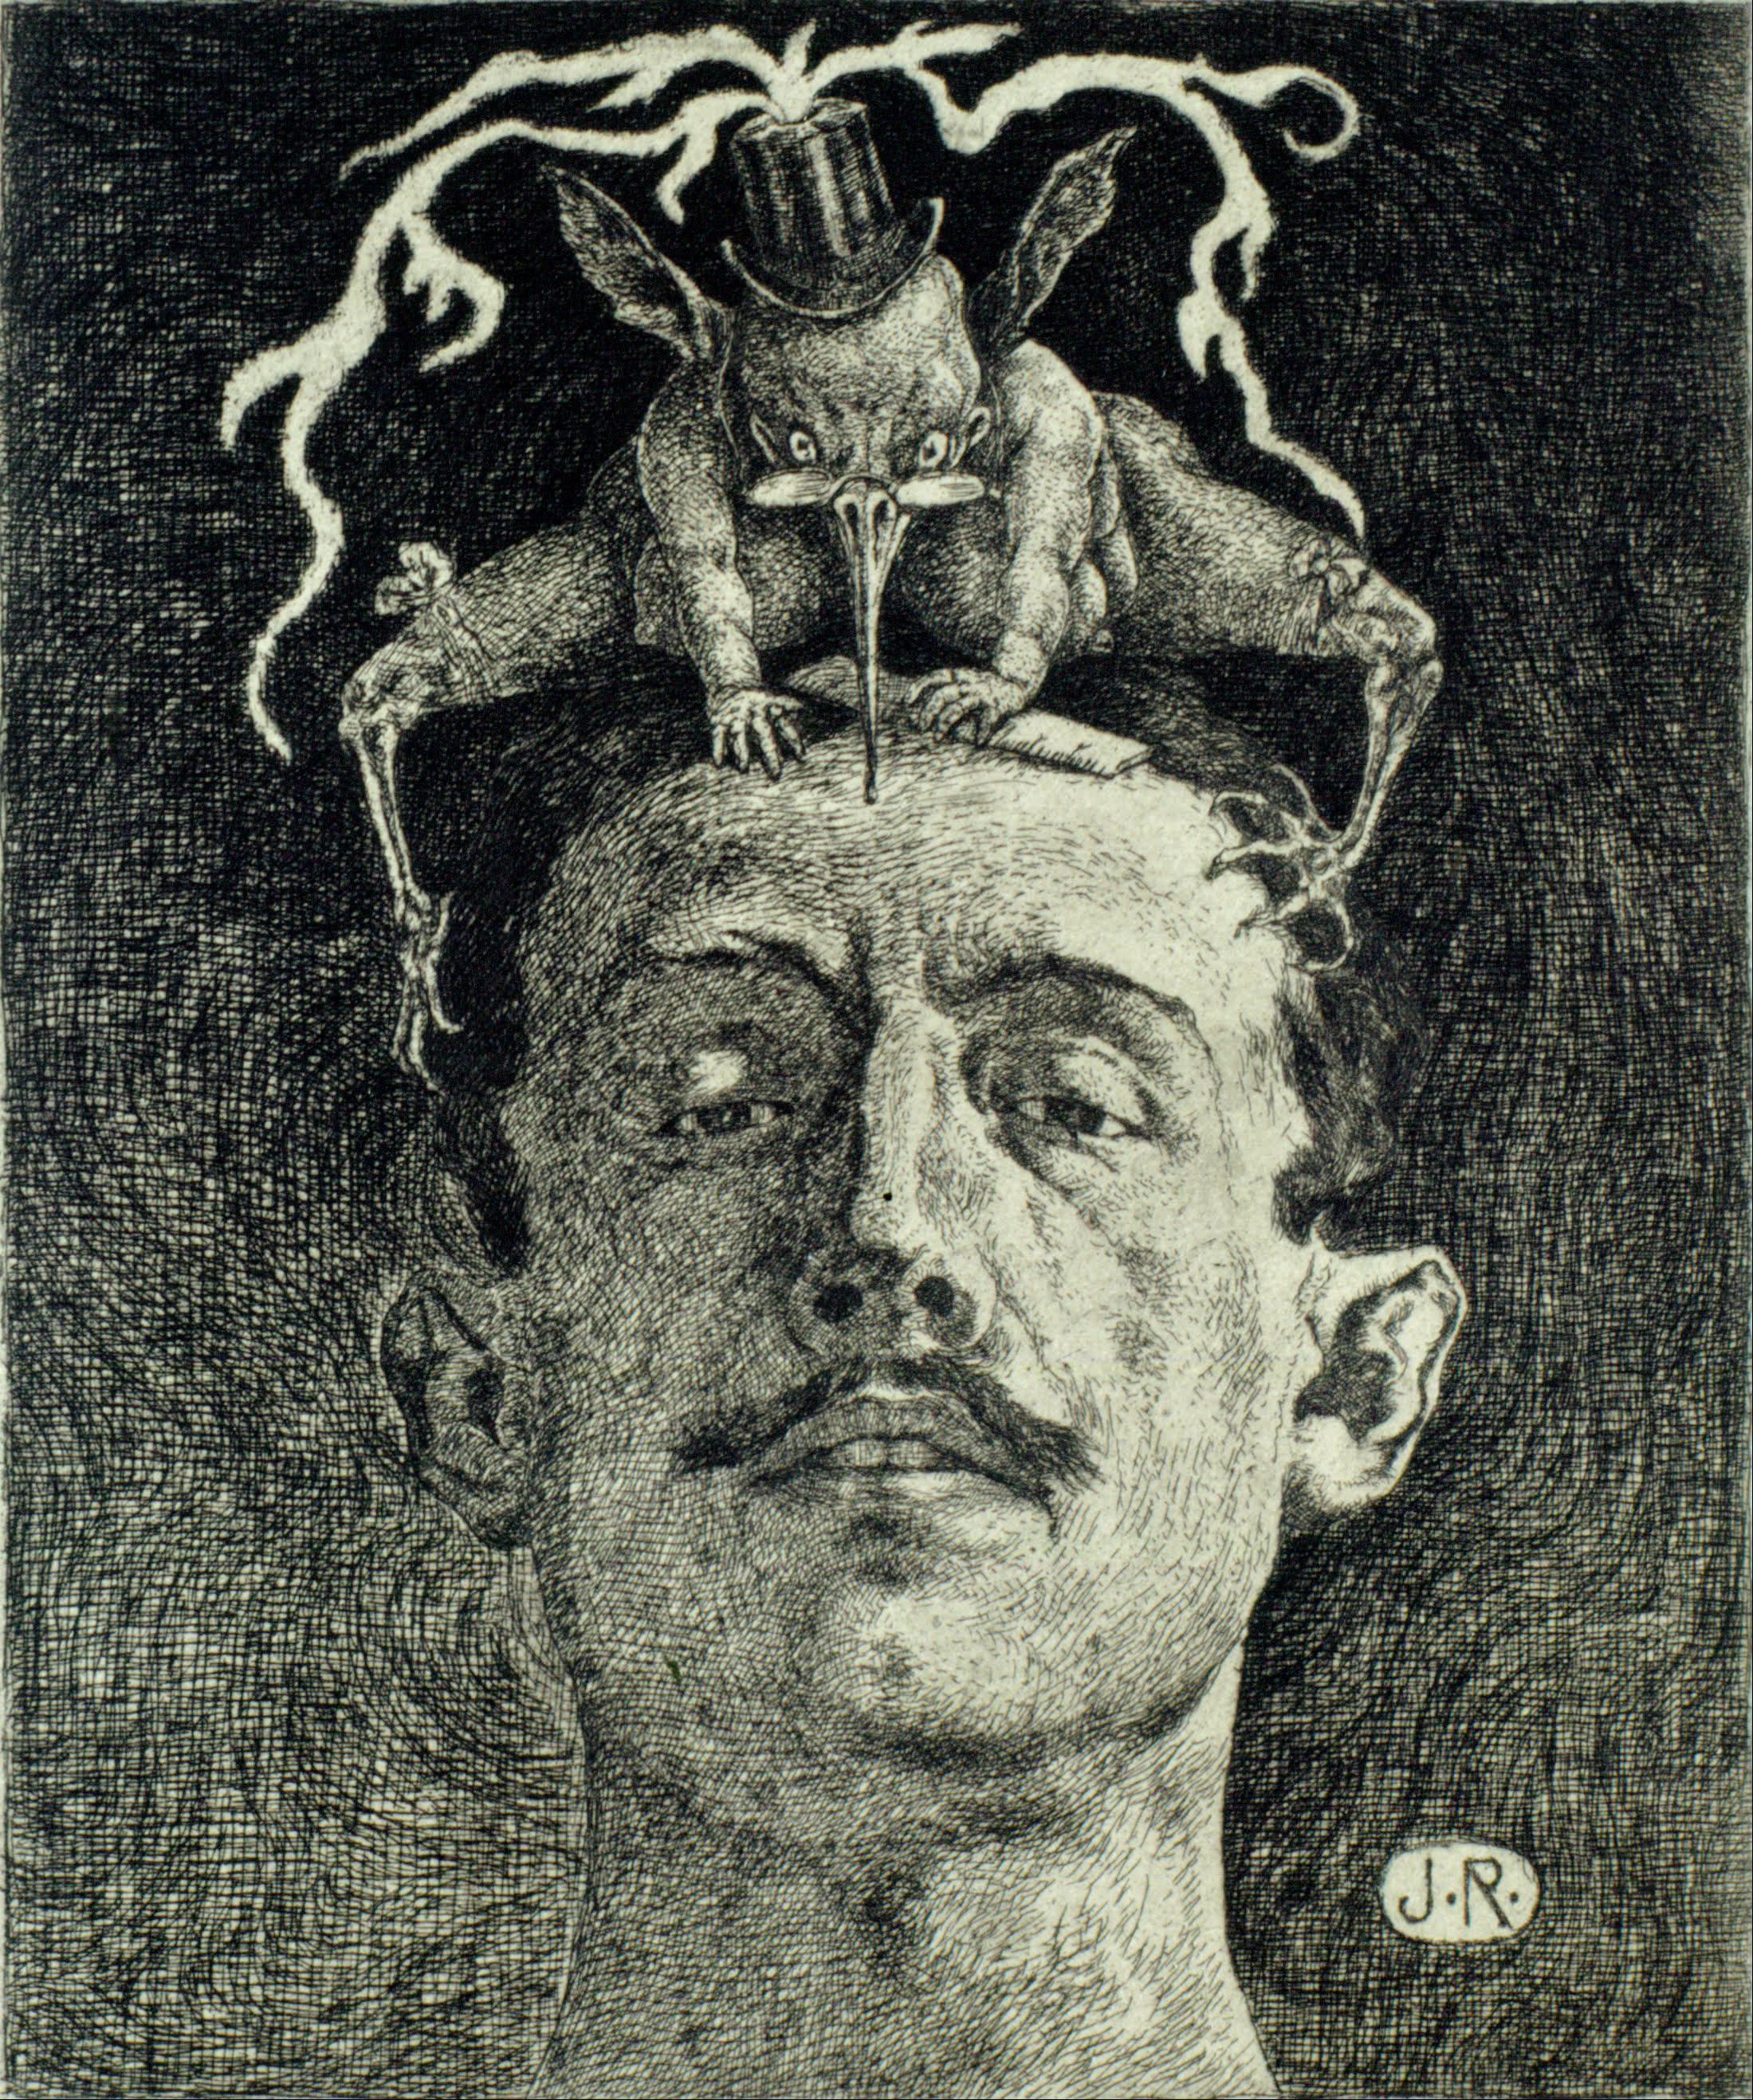
\includegraphics[width=0.3\textwidth]{innercritic}
  }
  \caption{Crítica by Julio Ruelas (ca. 1907). This artwork symbolizes the adversarial relationship central to GANs, where the critic (discriminator) evaluates the work of the creator (generator).}
\end{figure}
\vspace{0.5cm}

Generative Adversarial Networks (GANs) represent a groundbreaking approach in machine learning that has revolutionized generative modeling since their introduction in 2014. This thesis presents a comprehensive survey of the mathematical foundations underlying GANs, examining them through three complementary theoretical lenses: game theory, information theory, and optimal transport theory. By synthesizing these perspectives, we aim to provide a unified understanding of the principles that govern GAN behavior, training dynamics, and performance characteristics.

At its core, the GAN algorithm trains two neural networks through an adversarial two-player, zero-sum game. The first network, called the \textit{generator}, learns to produce synthetic data that resembles real samples from a target distribution. The second network, called the \textit{discriminator}, learns to distinguish between real data samples and those generated by the first network. This adversarial framework creates a dynamic where both networks improve in response to each other's progress, leading to increasingly realistic generated samples.

\subsection{Mathematical Framework of GANs}

The mathematical foundation of GANs begins with formal definitions of the generator and discriminator networks.

\begin{definition}%
  \label{def:generator}
  Let $\Phi \subset \mathbb{R}^n$ be a parameter space and $(\mathcal{Z}, p_z)$ be a prior probability space. A \textnormal{\sffamily generator} $G$ is a function $G: \Phi \times \mathcal{Z} \mapsto \mathcal{X}$ that maps a noise vector $z \sim p_z$ to the target space $(\mathcal{X}, p_{data})$. We denote the generator parameterized by $\phi \in \Phi$ as $G_\phi$.
\end{definition}

The generator transforms random noise from a simple prior distribution into complex samples that ideally follow the target data distribution. This transformation is parameterized by $\phi$, which is optimized during training to minimize the discrepancy between generated and real data distributions.

\begin{definition}%
  \label{def:discriminator}
  Let $\Theta \subset \mathbb{R}^m$ be a parameter space. A \textnormal{\sffamily discriminator} $D$ is a function $D: \Theta \times \mathcal{X} \mapsto [0, 1]$ that computes the probability that a sample $x \in \mathcal{X}$ was drawn from the real data distribution $(\mathcal{X}, p_{data})$ rather than the generator's distribution. We denote the discriminator parameterized by $\theta \in \Theta$ as $D_\theta$.
\end{definition}

The discriminator acts as a binary classifier that learns to distinguish between real and synthetic samples. Its output represents the estimated probability that a given sample originated from the real data distribution rather than being generated by $G_\phi$.

\begin{definition}
  The \textnormal{\sffamily Generative Adversarial Network} algorithm trains two neural networks in an adversarial manner:
  \begin{itemize}
    \item A generator $G_\phi$ that produces samples from the target space $(\mathcal{X}, p_{data})$
    \item A discriminator $D_\theta$ that estimates the probability that a sample came from $(\mathcal{X}, p_{data})$
  \end{itemize}
  
  The training process can be visualized as:
  \begin{center}
    \begin{tikzcd}
      \mathcal{Z} \arrow{r}{G_\phi} & \tilde{\mathcal{X}} \arrow{r}{} & (\mathcal{X}, \tilde{\mathcal{X}}) \arrow{r}{D_\theta} & [0, 1] \arrow{r}{V} & \mathbb{R} \\
      & \mathcal{X} \arrow{ur}{} & & &
    \end{tikzcd}
  \end{center}
  
  The discriminator maximizes and the generator minimizes the value function:
  \begin{align}
    \label{eq:intro-V}
    V(G_\phi, D_\theta) = \mathbb{E}_{x \sim p_{data}}[\log D_\theta(x)] + \mathbb{E}_{z \sim p_z}[\log(1 - D_\theta(G_\phi(z)))],
  \end{align}
  leading to the minimax optimization problem:
  \begin{align}
    \min_{\phi} \max_{\theta} V(G_\phi, D_\theta)
  \end{align}
\end{definition}

This adversarial formulation creates a dynamic equilibrium where the generator improves its ability to create realistic samples while the discriminator becomes more adept at detecting fakes. Ideally, this process converges when the generator produces samples indistinguishable from real data, forcing the discriminator to output approximately 0.5 for all inputs.

\subsection{Applications and Significance}

GANs have demonstrated remarkable success across numerous domains. In computer vision, they generate photo-realistic images of faces, objects, and scenes that are often indistinguishable from real photographs. Beyond image synthesis, GANs have found applications in:

\begin{itemize}
  \item \textbf{Medical Imaging}: Addressing class imbalance by generating synthetic images of rare conditions~\cite{ref:nazki-2018,ref:valerio-2017,ref:frid-2018} and enabling data anonymization for privacy-preserving research~\cite{ref:shin-2018}
  
  \item \textbf{Data Augmentation}: Creating additional training samples to improve model robustness, particularly in domains with limited real data
  
  \item \textbf{Anomaly Detection}: Leveraging the discriminator as a specialized classifier for identifying unusual patterns~\cite{ref:cortes-2017,ref:odena-2016}
  
  \item \textbf{Domain Adaptation}: Transferring knowledge between related domains by learning mappings between their distributions
\end{itemize}

While most research focuses on the generative capabilities, the discriminator component itself is a powerful binary classifier that has been successfully applied in various classification tasks, demonstrating the dual utility of the GAN framework.

\subsection{Neural Networks as Function Approximators}

Both the generator and discriminator in GANs are typically implemented as artificial neural networks, which serve as universal function approximators.

\begin{definition}
  A \textnormal{\sffamily Feedforward Neural Network} is a directed acyclic graph where each node computes a composition of an affine transformation followed by a nonlinear activation function. The network's behavior is determined by its connectivity structure and the parameters at each node.
\end{definition}

\begin{figure}[H] \centering
  \begin{tikzpicture} \tiny
    %%% Nodes.
    \begin{scope}[]
      \matrix[nodes = {draw, circle, minimum size=6mm, inner sep=0pt}, column sep = 0.5cm] {
        \node (q1) {$q_1$}; &
        \node (q2) {$q_2$}; &
        \node (q3) {$q_3$}; &
        \node (q4) {$q_4$}; &
        \node (q5) {$q_5$}; \\
      };
    \end{scope}
    \begin{scope}[yshift = -1cm]
      \matrix[nodes = {draw, circle, minimum size=6mm, inner sep=0pt}, column sep = 0.5cm] {
        \node (r1) {$r_1$}; &
        \node (r2) {$r_2$}; &
        \node (r3) {$r_3$}; &
        \node (r4) {$r_4$}; \\
      };
    \end{scope}
    \begin{scope}[yshift = -2cm]
      \matrix[nodes = {draw, circle, minimum size=6mm, inner sep=0pt}, column sep = 0.5cm] {
        \node (s1) {$s_1$}; &
        \node (s2) {$s_2$}; &
        \node (s3) {$s_3$}; & \node (s4) {$s_4$}; \\
      };
    \end{scope}
    \begin{scope}[yshift = -3cm]
      \matrix[nodes = {draw, circle, minimum size=6mm, inner sep=0pt}, column sep = 0.5cm] {
        \node (x1) {$x_1$}; &
        \node (x2) {$x_2$}; &
        \node (x3) {$x_3$}; &
        \node (x4) {$x_4$}; \\
      };
    \end{scope}
    \begin{scope}[yshift = -4cm]
      \matrix[nodes = {draw, circle, minimum size=6mm, inner sep=0pt}, column sep = 0.5cm] {
        \node (y1) {$y_1$}; &
        \node (y2) {$y_2$}; &
        \node (y3){$y_3$}; \\
      };
    \end{scope}
    \begin{scope}[yshift = -5cm]
      \matrix[nodes = {draw, circle, minimum size=6mm, inner sep=0pt}, column sep = 0.5cm] {
        \node (z1) {$z_1$}; &
        \node (z2) {$z_2$}; &
        \node (z3) {$z_3$}; &
        \node (z4) {$z_4$}; &
        \node (z5) {$z_5$}; \\
      };
\end{scope}
%%% Edges.
\foreach \q in {1, 2, 3, 4, 5} {
  \foreach \r in {1, 2, 3, 4} {
    \path [line] (q\q) -- (r\r);
  }
}
\foreach \r in {1, 2, 3, 4} {
  \foreach \s in {1, 2, 3, 4} {
    \path [line] (r\r) -- (s\s);
  }
}
\foreach \s in {1, 2, 3, 4} {
  \foreach \x in {1, 2, 3, 4} {
    \path [line] (s\s) -- (x\x);
  }
}
\foreach \x in {1, 2, 3, 4} {
  \foreach \y in {1, 2, 3} {
    \path [line] (x\x) -- (y\y);
  }
}
\foreach \y in {1, 2, 3} {
  \foreach \z in {1, 2, 3, 4, 5} {
    \path [line] (y\y) -- (z\z);
  }
}
  \end{tikzpicture}
  \caption{A deep neural network architecture showing multiple layers of interconnected nodes. Each node computes a weighted sum of inputs followed by a nonlinear activation function, enabling the network to approximate complex transformations.}
  \label{fig:deep_nn}
\end{figure}

If we denote a neural network parameterized by $\theta \in \Theta \subset \mathbb{R}^n$ as $f_\theta$, training involves searching the parameter space $\Theta$ for values that minimize a differentiable loss function $\mathcal{L}$. This optimization process typically uses gradient-based methods, where gradients are computed efficiently using the backpropagation algorithm~\cite{ref:rumelhart-1986}.

At each node, the computation typically follows the form:
\begin{align}
\sigma\left(\sum_{i=1}^n x_i\theta_i + b\right),
\end{align}
where $\sigma$ is a nonlinear activation function (e.g., sigmoid, ReLU), $\theta_i$ are weights, and $b$ is a bias term. This structure resembles a linear regression model:
\begin{align}
  \label{eq:lin-reg} \hat{y} = \sum_{i=1}^n x_i\theta_i + b,
\end{align}
but with the crucial addition of nonlinearity and composition across multiple layers. This hierarchical composition enables neural networks to approximate arbitrarily complex functions~\cite{ref:cheng-2018}.

\subsection{Historical Context and Theoretical Foundations}

The conceptual foundations of GANs draw from several historical threads in machine learning and game theory. An early precursor can be found in Doyle's work~\cite{ref:doyle}, which described a two-player game where one player selects a distribution and an adversary selects the "real" distribution, with the first player paying based on their surprise at observed outcomes. This framework shares the adversarial spirit of GANs, though without the formal optimization procedure.

In the 1990s, Schmidhuber introduced \textit{predictability minimization}~\cite{ref:schmidhuber-1992,ref:schmidhuber-2018}, where one network attempts to predict outcomes while an adversary tries to minimize this predictability. This adversarial training approach closely parallels the GAN framework. Subsequent work by Niemitalo~\cite{ref:niemitalo-2010} described a GAN-like algorithm in a blog post, while Zhou~\cite{ref:zhou-2012} developed adversarial support vector machines.

The modern GAN framework was introduced by Goodfellow et al.~\cite{ref:goodfellow-original} in 2014, building on these concepts and providing a unified, scalable algorithm for training generative models. This work triggered an explosion of research in generative modeling, with numerous variants addressing limitations of the original formulation.

\subsection{Theoretical Perspectives}

This thesis examines GANs through three complementary theoretical frameworks:

\begin{enumerate}
  \item \textbf{Game Theory}: GANs are fundamentally formulated as a two-player, zero-sum game between generator and discriminator. Game theory provides tools to analyze equilibrium properties, convergence behavior, and strategic interactions between the networks.
  
  \item \textbf{Information Theory}: The value function in GANs can be interpreted through information-theoretic quantities like Kullback-Leibler divergence and Jensen-Shannon divergence. This perspective reveals connections between GAN training and information maximization principles.
  
  \item \textbf{Optimal Transport}: The original GAN formulation suffered from training instability and mode collapse. Optimal transport theory, particularly the Wasserstein distance, has provided theoretical insights and practical improvements to address these challenges.
\end{enumerate}

By integrating these perspectives, this thesis aims to provide a comprehensive understanding of the mathematical principles underlying GANs, offering both theoretical insights and practical implications for researchers and practitioners in the field.

%%% Local Variables:
%%% mode: latex
%%% TeX-master: "../thesis"
%%% End:
